\section{Simplicial homology}

\subsection{Introduction and prerequisite algebra}

Throughout Michaelmas term, we will develop the notion of homology: a way of associating sequences of algebraic objects (in our case, abelian groups) to other mathematical objects (in our case, topological spaces). Specifically, we look at calculating the $n$th homology group of a topological space, denoted $H_n(X)$. This group has particular properties which is of interest in topology, namely its invariance over homeomorphisms and its functoriality (that is, for a map $f:X \to Y$, we have a induced map $f_*: H_n(X) \to H_n(Y)$).

We have some prerequisite algebra to help with our homology.

\begin{definition}
  The \emph{free abelian group} on generators $\{e_\alpha\}_{\alpha \in A}$ is the group
  \[ \Z\langle \{e_\alpha\}\rangle = \left\{\sum_{\alpha \in A} n_\alpha e_\alpha: n_\alpha \in \Z,\;\text{finitely many $n_\alpha \neq 0$}\right\}. \]
  An element of $\Z\langle\{e_\alpha\}\rangle$ may be called a \emph{formal sum}.
\end{definition}


We have a notion of the direct product of groups, but for free abelian groups we have the restriction that formal sums must have finitely many non-zero elements. Thus, the direct product of infinite families of free abelian groups may not be free abelian. From this, we introduce the notion of \emph{direct sum}: let $\{A_i\}_{i \in I}$ be a family of abelian groups, then
\[ \bigoplus_{i \in I} A_i = \left\{(a_i)_{i \in I} \in \prod_{i \in I} A_i: \;\text{finitely many $a_i \neq e$}\right\}. \]
This construction allows us to ensure a free abelian group from any family of abelian groups.

\subsection{Graph homology}

Graph homology is first introduced as a motivating case of the generalised \emph{simplicial homology}.
We may describe a directed graph as a 4-tuple
\[ G = (V, E, \alpha, \tau) \]
where $V$ is are the vertices, $E \subset \mathcal P(V)$ is are the edges, and $\alpha, \tau: E \to V$ describes the inital and terminal vertices of an edge respectively.
For example, the directed cycle graph of length 3 may be described as follows:
\[ DC_3 = (\{v_1, v_2, v_3\}, \{\{v_1, v_2\}, \{v_2, v_3\}, \{v_1, v_3\}\}, \alpha, \tau) \]
with $\alpha(\{v_1, v_2\}) = v_1$, $\alpha(\{v_2, v_3\}) = v_2$, $\alpha(\{v_1, v_3\}) = v_3$, $\tau(\{v_1, v_2\}) = v_2$, $\tau(\{v_2, v_3\}) = v_3$, and $\tau(\{v_1, v_3\}) = v_1$.
To visualise a graph, we define the \emph{geometric realisation} $\lvert G \rvert$ of a graph $G$ as the quotient space
\[
  \lvert G \rvert = \frac{V \cup (E \times [0,1])}{\langle (e,0) \sim \alpha(e), (e,1) \sim \tau(e): e \in E  \rangle}.
\]
$DC_3$, as described above, has the following geometric realisation.

\begin{center}
  % https://tikzcd.yichuanshen.de/#N4Igdg9gJgpgziAXAbVABwnAlgFyxMJZARgBoAGAXVJADcBDAGwFcYk6B9YkAX1PUy58hFACZSo6nSat2tDqN78QGbHgJFyEqQxZtEnAMy8pMKAHN4RUADMAThAC2SLSBwQkxPrYfPEZNw9EUW8QeyckcUCXHkoeIA
  \begin{tikzcd}
    & v_1 \arrow[rdd] &                \\
    &                 &                \\
    v_3 \arrow[ruu] &                 & v_2 \arrow[ll]
  \end{tikzcd}
\end{center}

We now move to the homology groups of a graph $G$. First, we define the \emph{chain groups} of $G$.

\begin{definition}
  Let $G = (V, E, \alpha, \tau)$ be a graph as defined above. We define
  \[
    C_0(G) = \Z\langle V \rangle, \qquad
    C_1(G) = \Z\langle E \rangle
  \]
  to be the $0$th and $1$st \emph{chain group} of $G$, respectively.
\end{definition}

Next, we move to define a map between the chain groups.

\begin{definition}
  Let $G = (V,E, \alpha, \tau)$. The \emph{boundary map} of $G$ is a group homomorphism $\partial_G: C_1(G) \to C_0(G)$ defined by $e \mapsto \tau(e) - \alpha(e)$, extending linearly.
\end{definition}

By extending linearly, we mean $\partial_G(\sum_i n_i e_i) = \sum_i n_i \partial(e_i)$. Finally, we define the homology of $G$.

\begin{definition}
  Let $G = (V,E, \alpha, \tau)$. Then
  \[ H_0(G) = \coker \partial_G, \qquad H_1(G) = \ker \partial_G \]
  are the $0$th and $1$st \emph{homology group} of $G$, respectively.
\end{definition}

Note, for a function $f: A \to B$, $\coker f = B/\im f$.

\begin{proposition}
  Let $G = (V,E, \alpha, \tau)$ be a graph. Then
  \[ H_0(G) \cong \Z^{c(G)}, \qquad H_1(G) \cong \Z^{\lvert E \rvert - \lvert V \rvert + c(G)} \]
  where $c(G)$ denotes the number of connected components in $\lvert G \rvert$.
\end{proposition}

\begin{proof}
  Here we will introduce some notions that become more con\-crete in the follow\-ing section. We have $H_0(G) \cong C_0(G)/\im \partial_G$. That is, vertices $v_1, v_2 \in V$ lay within the same equivalence class if $v_1 - v_2 \in \im \partial_G$. By the definition of $\partial_G$, we see this to be true if $v_1$ and $v_2$ are connected. Thus we assert that the rank of $H_0(G)$ must equal the number of connected components within $G$. Now, $H_1(G) \cong \ker \partial_G$: the cycles of $G$ ($e_1, \ldots, e_n$ is a cycle in $G$ if and only if $\partial_G(e_1 + e_2 + \ldots + e_n) = 0$). We first assume that $G$ is connected and let $T$ be a spanning tree. Observe that there exists a bijection between $E \setminus T$ and the set of linearly independent cycles of $G$. Thus $H_1(G) \cong \Z^{\lvert E \setminus T \rvert} = \Z^{\lvert E \rvert - (\lvert V \rvert - 1)} = \Z^{\lvert E \rvert - \lvert V \rvert + 1}$. A similar argument may extend this to a disconnceted graph to show $H_1(G) \cong \Z^{\lvert E \rvert - \lvert V \rvert + c(G)}$.
\end{proof}

\subsection{Simplicial homology}

We move to generalise graph homology to $n$-dimensions. We may recall the $n$-simplex, the generalisation of a point, line segment, triangle, etc. to arbitrary dimensions.

\begin{definition}
  We define the \emph{standard $n$-simplex} $\Delta^{n} \subset \R^{n+1}$ as
  \[ \Delta^n = \left\{\bm x = (x_0, \ldots, x_n) \in \R^{n+1}: \sum_{i = 0}^{n} x_i = 1\right\} \]
  with the subspace topology from $\R^{n+1}$.
\end{definition}

We move to a more abstract notion of a simplex, a family of sets that is closed under taking subsets but we weaken the notion of being tied to a specific space (although this notion is still there). We may denote such a simplex by an ordered list of vertices, note this induces an orientation on the faces. For example, $[v_0, v_1, v_2]$ may denote a $2$-simplex (a triangle).

\begin{definition}
  Let $\Delta^n = [v_0, \ldots, v_n]$ be a $n$-simplex. A \emph{face} of $\Delta^n$ is the $(n-1)$ simplex obtained from $\Delta^n$ by removing a vertex.
\end{definition}

Now we introduce a class of topological spaces called $\Delta$-complexes.

\begin{definition}
  A $\Delta$-structure on a topological space $X$ is a collection of maps $\{\sigma_\alpha\}_{\alpha \in I}$ where for each $\alpha \in I$, $\sigma_\alpha: \Delta^n \to X$ for some $n \in \N_0$. The collection must satisfy the following.
  \begin{enumerate}
    \item For each $\alpha \in I$, $\restr{\sigma_\alpha}{\mathring \Delta^n}$ is injective.
    \item For all $x \in X$, there is $\alpha \in I$ and $y \in \Delta^n$ such that $x = \sigma_\alpha(y)$.
    \item For each $\alpha \in I$, the restriction of $\sigma_\alpha$ to a face of $\Delta^n$ is $\sigma_\beta$ for some $\beta \in I$.
    \item $A \subset X$ is open if and only if $\sigma_\alpha^{-1}(A)$ is open for all $\alpha \in I$.
    \item Let $(\rho, \R^{n+1})$ be the permutation representation of $S_{n+1}$. Then for all $\alpha \in I$, there exists $\beta \in I$ such that $\sigma_\alpha = \sigma_\beta \circ \rho(\tau)$.
  \end{enumerate}
\end{definition}

A $\Delta$-complex is similar to a simplicial complex in the sense that we construct it by \emph{gluing} simplices together, but the rules of gluing are more lax for a $\Delta$-complex. Figure \ref{fig:delta-structures} shows some examples of $\Delta$-structures on the torus, projective plane, and klein bottle.

\begin{figure*}
  \centering
  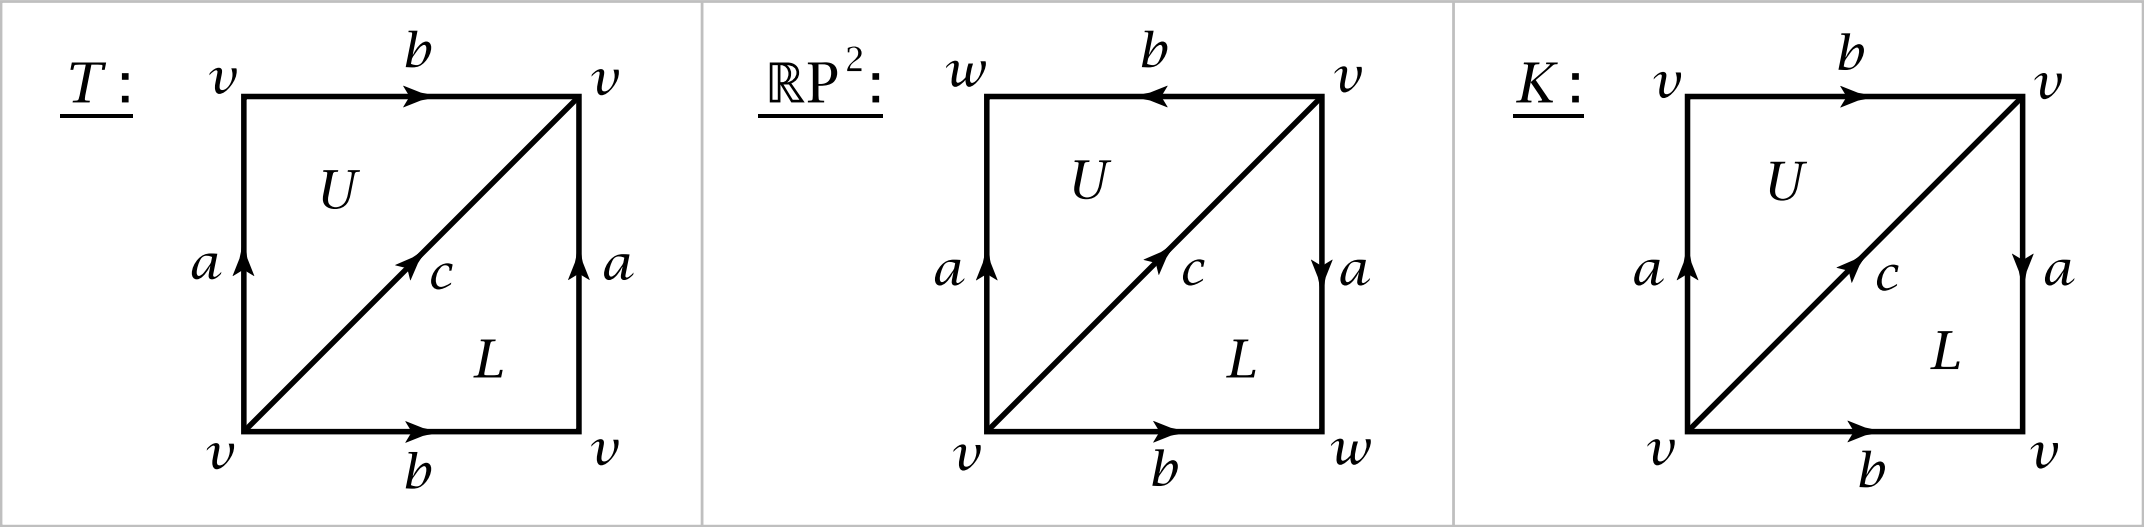
\includegraphics[width=\textwidth]{content/images/topic-1-1.png}
  \caption{Some examples of $\Delta$-structures for common topological spaces.}
  \label{fig:delta-structures}
\end{figure*}

We now move to define the chain groups and homology groups on a $\Delta$-complex much like we did for graphs.

\begin{definition}
  Let $X$ be a $\Delta$-complex. For $n \in \N_0$ where $\lvert \{ \sigma_\alpha^n \in X \} \rvert \neq 0$, we define the $n$th chain group of $X$ as
  \[C_n^\text{simp}(X) = \frac{\Z\langle \sigma_\alpha^n \in X \rangle}{\langle \sigma_\alpha^n \sim \sign(\tau) \sigma^n_\alpha \circ \rho(\tau): \tau \in S_{n+1}, \sigma_\alpha \in X \rangle}\]
  where $(\rho, \R^{n+1})$ is the permutation representation of $S_{n+1}$. When $\lvert \{ \sigma_\alpha^n \in X \} \rvert = 0$ (that is, there are no $n$-simplices) we define $C_n^\text{simp} (X) = 0$.
\end{definition}

Here we are identifying all simplices with the ordering of their vertices permuted (with an appropriate sign) as it is clear that $[v_0, v_1, v_2, \ldots, v_n]$ and $[v_1, v_0, v_2, \ldots, v_n]$ represent the same simplex (the sign of the permutation accounts for the orientation).

We now move to define a boundary map between adjacent chain groups, as we did between the $1$st and $0$th chain groups in graph homology.

\begin{definition}
  Let $X$ be a $\Delta$-complex and $n \in \N$. If $C_n^\text{simp}, C_{n-1}^\text{simp} \neq 0$, we define the $n$th boundary map as the group homomorphism
  \begin{align*}
    \partial_n^\text{simp}: C_n^\text{simp} & \to C_{n-1}^\text{simp},                                         \\
    [v_0, \ldots, v_n]                      & \mapsto \sum_{i=0}^n (-1)^i [v_0, \ldots, \hat v_i, \ldots, v_n]
  \end{align*}
  and extending linearly. When $C_n^\text{simp}$ or $C_{n-1}^\text{simp}$ are empty, then we define $\partial_n$ to be the zero homomorphism. We define $\partial_0$ to be the zero homomorphism too.
\end{definition}

For brevity, we use the notation
\[ [v_0, \ldots, \hat v_i, \ldots, v_n] = [v_0, \ldots, v_{i-1}, v_{i+1}, \ldots, v_n]. \]
Note that $C_n^\text{simp}$ is the free abelian group on generators being the $n$-simplices (where two simplices with the same vertex set permuted are identified graded by the sign of the permutation), so we must extended linearly for $\partial_n^\text{simp}$ to be well defined. Formally, we mean:
\[
  \partial_n^\text{simp}\left(\sum_\alpha n_\alpha \sigma_\alpha\right) = \sum_\alpha n_\alpha \partial_n^\text{simp} (\sigma_\alpha).
\]
To motivate the alternating sum: we want to preserve orientation of our vertices (as given to our chain group in the definition of $C_n^\text{simp}(X)$). 

The natural next step, after following the special case of graph homology, would be to move onto defining the homology groups as the quotients $\ker \delta_n/\im \delta_{n+1}$, but first we need to ensure this quotient is well-defined. Indeed, all subgroups of abelian groups are normal, but we must ensure that $\im \delta_{n+1} \subset \ker \delta_n$. This motivates the following lemma.

\begin{lemma}
  Let $\{\partial_n^\text{simp}\}_{n \in \N_0}$ be the boundary maps of a $\Delta$-complex. Then for all $n \in \N$,
  \[ \partial_{n-1}^\text{simp} \circ \partial_{n}^\text{simp} = 0. \]
\end{lemma}

\begin{proof}
  Trivially, $\partial_0^\text{simp} \circ \partial_1^\text{simp} = 0 \circ \partial_1^\text{simp} = 0$. We let $n \in \{2, 3, \ldots\}$. Let $\sigma = [v_0, v_1, \ldots, v_n]$ a $n$-simplex. Then we have \[\partial_n(\sigma) = \sum_{i=0}^n (-1)^i [v_0, \ldots, \hat v_i, \ldots, v_n].\] Thus
  \begin{align*}
    (\partial_{n-1} \circ \partial_n)(\sigma) & = \partial_{n-1} \left(\sum_{i=0}^n (-1)^i [v_0, \ldots, \hat v_i, \ldots, v_n]\right)                     \\
                                              & = \sum_{i=0}^n (-1)^i \partial_{n-1}([v_0, \ldots, \hat v_i, \ldots, v_n])                                 \\
                                              & = \sum_{i < j} (-1)^i (-1)^{j-1} \partial_{n-1}([v_0, \ldots, \hat v_i, \ldots, \hat v_j, \ldots, v_n])\,+ \\ &\qquad\qquad \sum_{j < i} (-1)^i (-1)^{j} \partial_{n-1}([v_0, \ldots, \hat v_j, \ldots, \hat v_i, \ldots, v_n]) \\
                                              & = 0.
  \end{align*}
  We can see that the two summations cancel after switching $i$ and $j$ in either summation, it becomes the negative of the first.
\end{proof}

We are now comfortable defining our homology groups.

\begin{definition}
  Let $X$ be a $\Delta$-complex with boundary maps $\{\partial_n^\text{simp}: C_n^\text{simp} \to C_{n-1}^\text{simp}\}_{n \in \N_0}$. For $n \in \N_0$, we define the $n$th \emph{simplicial homology group} of $X$ as
  \[ H_n^\text{simp}(X) = \frac{\ker\partial_n^\text{simp}}{\im\partial_{n+1}^\text{simp}}. \]
\end{definition}

We will look to calculate the simplicial homology groups on the three $\Delta$-com\-plex\-es introduced in Figure \ref{fig:delta-structures}.

\begin{example}
   For the $\Delta$-complex on the torus, we get the following simplicial chain complex.
  \begin{center}
    % https://tikzcd.yichuanshen.de/#N4Igdg9gJgpgziAXAbVABwnAlgFyxMJZABgBpiBdUkANwEMAbAVxiRAGEB9AJgD0AdfjhgAPHMGwBbNAF8AFAA0AlCBml0mXPkIoAjOSq1GLNl10Cho8VNmKVajdjwEi3A9XrNWiDp2IXhMQksaXllVXUQDCdtIgBmdyMvNmIIxy0XFDJdQ08TH0FJOhwACwAjMoACAC1ebjSozWcdZH0cj2NvEELi8qrauIbojJa3dqT87v4i0oqa1UMYKABzeCJQADMAJwhJJDIQHAgkfQmuwTQ6LbxGHhBqBjoymAYABSbYny2sZZKcBu2uxO1COSDcZzYFyuNwYnF09xAj2ebw+mRA31+-wcIEBe0Q4NBiASEIK-Eu1ywt1SDyeL3eMTRGL+AJ2eIOhIALB1kqSAMYEZYsoGIU6EgCs3Mmgn5YEF2NxYJBx0QADZJed+DK5ZEFYguYdlRKSSAALJ3eWspBGwlq41m+EyCgyIA
    \begin{tikzcd}
      C_2^\text{simp}(X) \arrow[r, "\partial_2"'] \arrow[d, "\cong"] & C_1^\text{simp}(X) \arrow[r, "\partial_1"'] \arrow[d, "\cong"] & C_0^\text{simp}(X) \arrow[r, "\partial_0"'] \arrow[d, "\cong"] & 0 \\
      \mathbb Z^2 \arrow[r, "M_2"]                                   & \mathbb Z^3 \arrow[r, "M_1"]                                   & \mathbb Z                                                      &
    \end{tikzcd}
  \end{center}
  where
  $
    M_2 =
    \begin{pmatrix}
      1 & -1 \\ 1 & -1 \\ -1 & 1
    \end{pmatrix}
  $
  and
  $
    M_1 =
    \begin{pmatrix}
      0 & 0 & 0
    \end{pmatrix}
  $.
  Thus we get
  \[
    H_n(X) =
    \begin{cases}
      \Z   & n = 0, 2,         \\
      \Z^2 & n = 1,            \\
      0    & \text{otherwise}.
    \end{cases}
  \]
  \end{example}

\begin{example}
   For the $\Delta$-complex on the real projective plane, we have the following simplicial chain complex.
  \begin{center}
    % https://tikzcd.yichuanshen.de/#N4Igdg9gJgpgziAXAbVABwnAlgFyxMJZABgBpiBdUkANwEMAbAVxiRAGEB9AJgD0AdfjhgAPHMGwBbNAF8AFAA0AlCBml0mXPkIoAjOSq1GLNl10Cho8VNmKVajdjwEi3A9XrNWiDp2IXhMQksaXllVXUQDCdtIgBmdyMvNmIIxy0XFDJdQ08TH0FJOhwACwAjMoACAC1ebjSozWcdZH0cj2NvEELi8qrauIbojJa3dqT87v4i0oqautVDGCgAc3giUAAzACcISSQyEBwIJH0JrsE0Om28Rh4QagY6MpgGAAUm2J9trBWSnAaOz2p2oxyQbnObEu11uDE4ugeICeL3en0yIB+fwBDhAQP2iAhYMQCUhBX4VxuWDuqUez1eHxi6Mx-0Bu3xhyJABYOskyQBjAgrVnAxBnIkAVh5k0EArAQpxePBoJOiAAbFKLvxZfLIorENyjirJaSQABZe4KtlIY1E9Um80ImQUGRAA
    \begin{tikzcd}
      C_2^\text{simp}(X) \arrow[r, "\partial_2"'] \arrow[d, "\cong"] & C_1^\text{simp}(X) \arrow[r, "\partial_1"'] \arrow[d, "\cong"] & C_0^\text{simp}(X) \arrow[r, "\partial_0"'] \arrow[d, "\cong"] & 0 \\
      \mathbb Z^2 \arrow[r, "M_2"]                                   & \mathbb Z^3 \arrow[r, "M_1"]                                   & \mathbb Z^2                                                    &
    \end{tikzcd}
  \end{center}
  where
  $
    M_2 =
    \begin{pmatrix}
      -1 & -1 \\ 1 & 1 \\ 1 & -1
    \end{pmatrix}
  $
  and
  $
    M_1 =
    \begin{pmatrix}
      -1 & -1 & 0 \\
      1  & 1  & 0
    \end{pmatrix}
  $.
  Thus we get
  \[
    H_n(X) =
    \begin{cases}
      \Z   & n = 0,            \\
      \Z_2 & n = 1,            \\
      0    & \text{otherwise}.
    \end{cases}
  \]
\end{example}

\begin{example}
 For the $\Delta$-complex on the klein bottle, we have the following simplicial chain complex.
  \begin{center}
    % https://tikzcd.yichuanshen.de/#N4Igdg9gJgpgziAXAbVABwnAlgFyxMJZABgBpiBdUkANwEMAbAVxiRAGEB9AJgD0AdfjhgAPHMGwBbNAF8AFAA0AlCBml0mXPkIoAjOSq1GLNl10Cho8VNmKVajdjwEi3A9XrNWiDp2IXhMQksaXllVXUQDCdtIgBmdyMvNmIIxy0XFDJdQ08TH0FJOhwACwAjMoACAC1ebjSozWcdZH0cj2NvEELi8qrauIbojJa3dqT87v4i0oqa1UMYKABzeCJQADMAJwhJJDIQHAgkfQmuwTQ6LbxGHhBqBjoymAYABSbYny2sZZKcBu2uxO1COSDcZzYFyuNwYnF09xAj2ebw+mRA31+-wcIEBe0Q4NBiASEIK-Eu1ywt1SDyeL3eMTRGL+AJ2eIOhIALB1kqSAMYEZYsoGIU6EgCs3Mmgn5YEF2NxYJBx0QADZJed+DK5ZEFYguYdlRKSSAALJ3eWspBGwlq41m+EyCgyIA
    \begin{tikzcd}
      C_2^\text{simp}(X) \arrow[r, "\partial_2"'] \arrow[d, "\cong"] & C_1^\text{simp}(X) \arrow[r, "\partial_1"'] \arrow[d, "\cong"] & C_0^\text{simp}(X) \arrow[r, "\partial_0"'] \arrow[d, "\cong"] & 0 \\
      \mathbb Z^2 \arrow[r, "M_2"]                                   & \mathbb Z^3 \arrow[r, "M_1"]                                   & \mathbb Z                                                      &
    \end{tikzcd}
  \end{center}
  where
  $
    M_2 =
    \begin{pmatrix}
      -1 & -1 \\ -1 & 1 \\ 1 & -1
    \end{pmatrix}
  $
  and
  $
    M_1 =
    \begin{pmatrix}
      0 & 0 & 0
    \end{pmatrix}
  $.
  Thus we get
  \[
    H_n(X) =
    \begin{cases}
      \Z             & n = 0,            \\
      \Z \oplus \Z_2 & n = 1,            \\
      0              & \text{otherwise}.
    \end{cases}
  \]

\end{example}